\documentclass[a4paper]{article}
\usepackage{a4wide}
\usepackage{graphicx}
\usepackage{pxfonts}
\usepackage{tikz}
\usepackage{calc}
\usepackage{ifthen}
\usepackage{listings}
\usepackage{url}
\usepackage{booktabs}
\usepackage{fourier}

\usetikzlibrary{calc,decorations.text,patterns,shapes.arrows,shapes,shadings,arrows,automata,positioning,shadows}

\pagestyle{empty}

\lstdefinelanguage{generic}{
  escapechar=@,%
  basicstyle={\ttfamily},%
  keywordstyle={\ttfamily\bfseries},%
  commentstyle={\it},%
  captionpos=b%
}

\lstdefinelanguage{JavaScript}{
  keywords={typeof, new, true, false, catch, function, return,
            null, catch, switch, var, if, in, for, while, do, else, case, break},
  keywordstyle=\color{blue}\bfseries,
  ndkeywords={class, export, boolean, throw, implements, import, this},
  ndkeywordstyle=\color{darkgray}\bfseries,
  identifierstyle=\color{black},
  sensitive=false,
  comment=[l]{//},
  morecomment=[s]{/*}{*/},
  basicstyle=\tt,
  commentstyle=\color{purple}\ttfamily,
  stringstyle=\color{red}\ttfamily,
  morestring=[b]',
  morestring=[b]",
  escapeinside=\`\`,
  columns=fullflexible
}

\renewcommand{\labelitemi}{\raisebox{1pt}{\danger}}

\newcommand{\PLACEHOLDER}[1]{\ensuremath{\langle}\textrm{\textit{#1}\ensuremath{\rangle}}}
\newcommand{\X}[2]{\tikz[baseline,remember picture]{\node[anchor=base,inner sep=0mm] (#2) {{#1}};}}
\newcommand{\V}[1]{\pgfkeysvalueof{#1}}
\newcommand{\examplecode}[2][.9\linewidth]{\begin{center}\begin{minipage}{#1}\lstinputlisting[language=javascript,frame=lines]{#2}\end{minipage}\end{center}}
\newcommand{\inlinecode}[2][]{\lstinputlisting[language=javascript,#1]{#2}}
\newcommand{\SECTION}[1]{
  \begin{center}
    \begin{tikzpicture}
      \node[section] { \Huge #1 };
    \end{tikzpicture}
  \end{center}
}
\newcommand{\SUBSECTION}[1]{
  \begin{center}
    \begin{tikzpicture}
      \node[subsection] { \Large #1 };
    \end{tikzpicture}
  \end{center}
}

\pgfkeys{tikz/section/.style={drop shadow,thick,rectangle,fill=gray,inner sep=2mm,minimum width=.9\textwidth,minimum height=1.5cm}}
\pgfkeys{tikz/subsection/.style={rectangle,fill=gray!50,text opacity=1,inner sep=2mm,minimum width=.8\textwidth,minimum height=1cm}}
\pgfkeys{tikz/item/.style={rectangle,fill=gray,opacity=0.25,text opacity=1,inner sep=2mm,minimum height=.75cm}}

\pgfkeys{/tikz/flowchart/node/.style={rectangle,fill=blue,opacity=0.5,text opacity=1,drop shadow,inner sep=2mm}}
\pgfkeys{/tikz/flowchart/arrow/.style={-latex,thick}}
\pgfkeys{/tikz/flowchart/arrowline/.style={thick}}


\begin{document}

\SECTION{{\tt if}-statement}

\SUBSECTION{Syntax}
\examplecode[.35\linewidth]{ifelse.js}

\SUBSECTION{Semantics}
\begin{center}
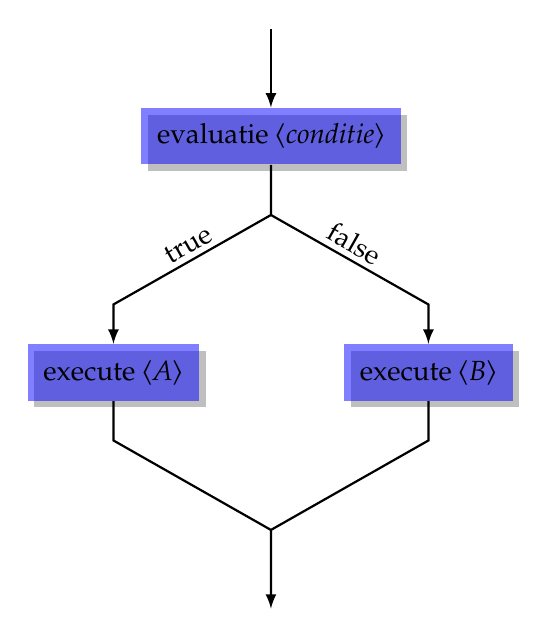
\begin{tikzpicture}
  \node[flowchart/node] (if) at (0,3) {evaluatie \PLACEHOLDER{conditie}};
  \node[flowchart/node] (then) at (-2, 0) {execute \PLACEHOLDER{A}};
  \node[flowchart/node] (else) at (2, 0) {execute \PLACEHOLDER{B}};

  \draw[flowchart/arrow] ($ (if.north) + (0,1) $) -- (if.north);
  \draw[flowchart/arrow] (if.south) -- (0,2) -- ($ (then.north) + (0,0.5) $) -- (then.north);
  \draw[flowchart/arrow] (0,2) -- ($ (else.north) + (0,0.5) $) -- (else.north);
  \path[flowchart/arrow,decorate,decoration={text along path,text={true},text align={align=center},reverse path}] (0, 2.1) -- ($ (then.north) + (0,0.6) $);
  \path[flowchart/arrow,decorate,decoration={text along path,text={false},text align={align=center}}] (0, 2.1) -- ($ (else.north) + (0,0.6) $);

  \draw[flowchart/arrow] (then.south) -- ($ (then.south) - (0,0.5) $) -- (0,-2) -- (0,-3);
  \draw[flowchart/arrowline] (else.south) -- ($ (else.south) - (0,0.5) $) -- (0,-2);
\end{tikzpicture}

\end{center}

\SUBSECTION{Remarks}
\begin{itemize}
  \item Make sure to distinguish comparison {\tt ===} from assignment {\tt =}. In a condition, you generally need the former.
  \item The {\tt else} is optional.
\end{itemize}


\clearpage
\SECTION{{\tt while}-statement}
\SUBSECTION{Syntax}
\examplecode[.35\linewidth]{while.js}

\SUBSECTION{Semantics}
\begin{center}
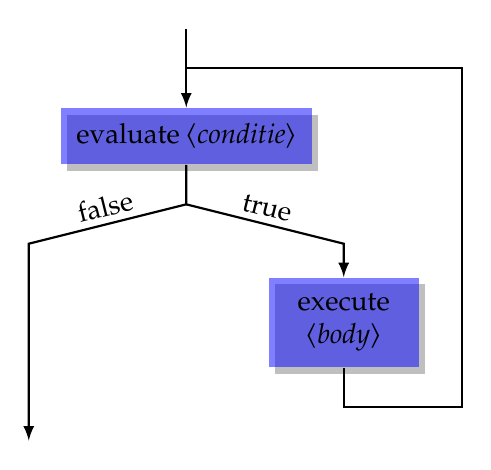
\begin{tikzpicture}
  \node[flowchart/node] (while) {evaluate \PLACEHOLDER{conditie}};
  \node (loop entry) at ($ (while.north) + (0,0.5) $) {};
  \node[flowchart/node] (body) at ($ (while.south) + (2,-2) $) {\parbox{1.5cm}{\centering execute \PLACEHOLDER{body}}};
  \node (split) at ($ (while.south) + (0,-0.5) $) {};

  \draw[flowchart/arrow] ($ (while.north) + (0,1) $) -- (while.north);
  \draw[flowchart/arrow] (while.south) -- (split.center) -- ++(-2,-0.5) -- ++(0,-2.5);
  \draw[flowchart/arrow] (split.center) -- ++(2,-0.5) -- (body.north);
  \draw[flowchart/arrowline] (body.south) -- ++(0,-0.5) -- ++(1.5,0) |- (loop entry.center);

  \path[flowchart/arrow,decorate,decoration={text along path,text={false},text align={align=center},reverse path}] ($ (while.south) + (0,-0.4) $) -- ++(-2,-0.5);
  \path[flowchart/arrow,decorate,decoration={text along path,text={true},text align={align=center}}] ($ (while.south) + (0,-0.4) $) -- ++(2,-0.5);
\end{tikzpicture}

\end{center}

\SUBSECTION{Remarks}
\begin{itemize}
  \item Make sure to distinguish comparison {\tt ===} from assignment {\tt =}. In a condition, you generally need the former.
  \item The {\tt while} has \emph{no} {\tt else}.
\end{itemize}


\clearpage
\SECTION{{\tt for}-statement}
\SUBSECTION{Syntax}
\examplecode[.35\linewidth]{for.js}

\SUBSECTION{Semantics}
\begin{center}
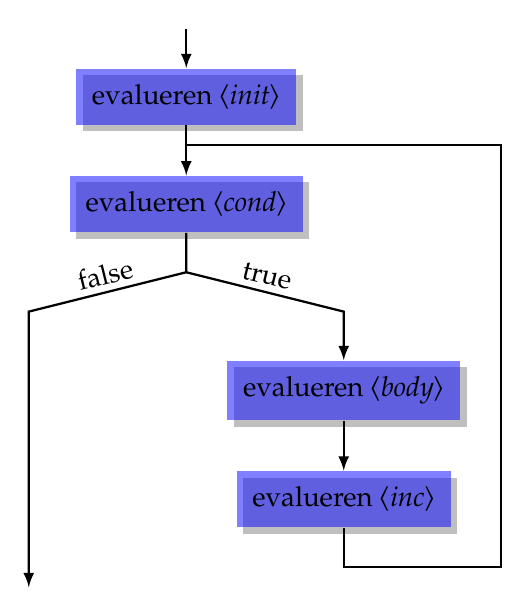
\begin{tikzpicture}
  \node[flowchart/node] (init) {evalueren \PLACEHOLDER{init}};
  \node (loop) at ($ (init.south) + (0,-0.25) $) {};
  \node[flowchart/node] (cond) at ($ (init.south) + (0,-1) $) {evalueren \PLACEHOLDER{cond}};
  \node (split) at ($ (cond.south) + (0,-0.5) $) {};
  \node[flowchart/node] (body) at ($ (split.center) + (2,-1.5) $) {evalueren \PLACEHOLDER{body}};
  \node[flowchart/node] (inc) at ($ (body.south) + (0,-1) $) {evalueren \PLACEHOLDER{inc}};

  \draw[flowchart/arrow] ($ (init.north) + (0,0.5) $) -- (init.north);
  \draw[flowchart/arrow] (init.south) -- (cond.north);
  \draw[flowchart/arrow] (cond.south) -- (split.center) -- ++(-2,-0.5) -- ++(0,-3.5);
  \draw[flowchart/arrow] (split.center) -- ++(2,-0.5) -- (body.north);
  \draw[flowchart/arrow] (body.south) -- (inc.north);
  \draw[flowchart/arrowline] (inc.south) -- ++(0,-0.5) -- ++(2,0) |- (loop.center);

  \path[flowchart/arrow,decorate,decoration={text along path,text={false},text align={align=center},reverse path}] ($ (split.center) + (0,.1) $) -- ++(-2,-0.5);
  \path[flowchart/arrow,decorate,decoration={text along path,text={true},text align={align=center}}] ($ (split.center) + (0,.1) $) -- ++(2,-0.5);
\end{tikzpicture}

\end{center}

\SUBSECTION{Remarks}
\begin{itemize}
  \item Make sure to distinguish comparison {\tt ===} from assignment {\tt =}. In a condition, you generally need the former.
  \item Don't forget to use {\tt var} in \PLACEHOLDER{init}, i.e.\ {\tt var i = 0} instead of just {\tt i = 0}.
\end{itemize}


\clearpage
\SECTION{Arrays}
\SUBSECTION{Syntax}

\begin{center}
  \begin{tikzpicture}
    \path[use as bounding box] (-5,.5) rectangle (5,-9);
    \node[anchor=east,item,minimum width=5cm] at (0,0) {Array creation with length $n$};
    \node[anchor=west] at (0.1,0) {\inlinecode{newarray.js}};
    \node[anchor=east,item,minimum width=5cm] at (0,-1) {Reading};
    \node[anchor=west] at (0.1,-1) {\inlinecode{readfromarray.js}};
    \node[anchor=east,item,minimum width=5cm] at (0,-2) {Writing};
    \node[anchor=west] at (0.1,-2) {\inlinecode{writetoarray.js}};
    \node[anchor=east,item,minimum width=5cm] at (0,-3) {Length};
    \node[anchor=west] at (0.1,-3) {\inlinecode{arraylength.js}};
    \node[anchor=east,item,minimum width=5cm] at (0,-4) {Add to end};
    \node[anchor=west] at (0.1,-4) {\inlinecode{arraypush.js}};
    \node[anchor=east,item,minimum width=5cm] at (0,-5) {Remove from end};
    \node[anchor=west] at (0.1,-5) {\inlinecode{arraypop.js}};
    \node[anchor=east,item,minimum width=5cm] at (0,-6) {Add to beginning};
    \node[anchor=west] at (0.1,-6) {\inlinecode{arrayunshift.js}};
    \node[anchor=east,item,minimum width=5cm] at (0,-7) {Remove from beginning};
    \node[anchor=west] at (0.1,-7) {\inlinecode{arrayshift.js}};
    \node[anchor=east,item,minimum width=5cm] at (0,-8) {Subarray};
    \node[anchor=west] at (0.1,-8) {\inlinecode{arrayslice.js}};
  \end{tikzpicture}
\end{center}

\SUBSECTION{Remarks}
\begin{itemize}
  \item Copying an array is easiest using {\tt xs.slice();}
  \item Array indices are \emph{zero-based}, i.e.\ the first element has index {\tt 0}, the last has index {\tt xs.length - 1}.
  \item For the exam:
        \begin{itemize}
          \item Only indexing and {\tt length} are allowed (meaning, no {\tt push}, {\tt pop}, {\tt slice}, \dots).
          \item You are \emph{not} allowed to read or write beyond an array's bounds.
        \end{itemize}
\end{itemize}


\clearpage
\SECTION{Objecten}
\SUBSECTION{Syntax}

\begin{center}
  \begin{tikzpicture}
    \path[use as bounding box] (-5,.5) rectangle (5,-5);
    \node[anchor=east,item,minimum width=5cm] at (0,0) {Creation empty object};
    \node[anchor=west] at (0.1,0) {\inlinecode{newobject.js}};
    \node[anchor=east,item,minimum width=5cm] at (0,-1) {Reading};
    \node[anchor=west] at (0.1,-1) {\inlinecode{readfromobject.js}};
    \node[anchor=east,item,minimum width=5cm] at (0,-2) {Reading (alternative syntax)};
    \node[anchor=west] at (0.1,-2) {\inlinecode{readfromobject2.js}};
    \node[anchor=east,item,minimum width=5cm] at (0,-3) {Writing};
    \node[anchor=west] at (0.1,-3) {\inlinecode{writetoobject.js}};
    \node[anchor=east,item,minimum width=5cm] at (0,-4) {Writing (alternative syntax)};
    \node[anchor=west] at (0.1,-4) {\inlinecode{writetoobject2.js}};

  \end{tikzpicture}
\end{center}

\SUBSECTION{Arrays vs Objects}
\begin{center}
  \begin{tabular}{lcc}
    & {\bf arrays} & {\bf objects} \\
    \toprule
    index & integers & strings \\[2mm]
    length & fixed & grows by need \\[2mm]
    querying length & {\tt length} & N/A \\
  \end{tabular}
\end{center}

\SUBSECTION{Remarks}
\begin{itemize}
  \item Objects are optional: you don't need to know them for the exam, but they
    can considerably simplify your life.
\end{itemize}


\clearpage
\SECTION{Operators}
\SUBSECTION{Comparison}
\begin{center}
  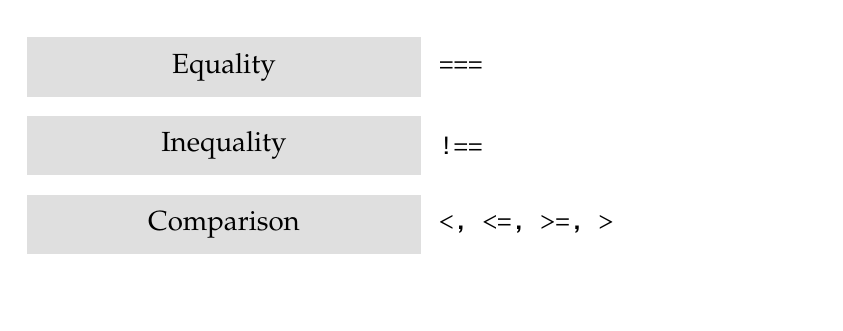
\begin{tikzpicture}
    \path[use as bounding box] (-5,.5) rectangle (5,-3);
    \node[anchor=east,item,minimum width=5cm] at (0,0) {Equality};
    \node[anchor=west] at (0.1,0) {\tt ===};
    \node[anchor=east,item,minimum width=5cm] at (0,-1) {Inequality};
    \node[anchor=west] at (0.1,-1) {\tt !==};
    \node[anchor=east,item,minimum width=5cm] at (0,-2) {Comparison};
    \node[anchor=west] at (0.1,-2) {\tt <, <=, >=, >};
  \end{tikzpicture}
\end{center}

\SUBSECTION{Arithmetic Operators}
\begin{center}
  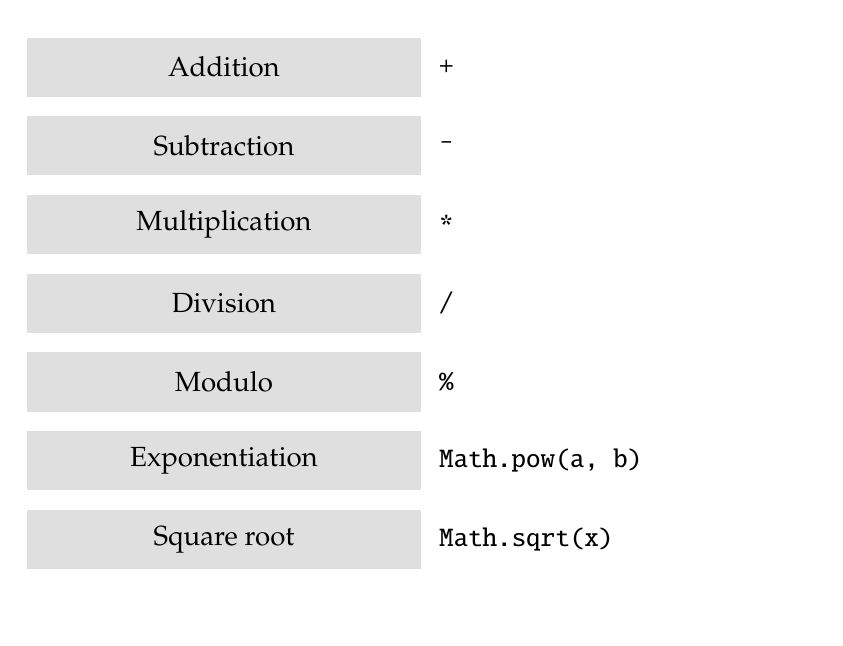
\begin{tikzpicture}
    \path[use as bounding box] (-5,.5) rectangle (5,-7);
    \node[anchor=east,item,minimum width=5cm] at (0,0) {Addition};
    \node[anchor=west] at (0.1,0) {\tt +};
    \node[anchor=east,item,minimum width=5cm] at (0,-1) {Subtraction};
    \node[anchor=west] at (0.1,-1) {\tt -};
    \node[anchor=east,item,minimum width=5cm] at (0,-2) {Multiplication};
    \node[anchor=west] at (0.1,-2) {\tt *};
    \node[anchor=east,item,minimum width=5cm] at (0,-3) {Division};
    \node[anchor=west] at (0.1,-3) {\tt /};
    \node[anchor=east,item,minimum width=5cm] at (0,-4) {Modulo};
    \node[anchor=west] at (0.1,-4) {\tt \%};
    \node[anchor=east,item,minimum width=5cm] at (0,-5) {Exponentiation};
    \node[anchor=west] at (0.1,-5) {\tt Math.pow(a, b)};
    \node[anchor=east,item,minimum width=5cm] at (0,-6) {Square root};
    \node[anchor=west] at (0.1,-6) {\tt Math.sqrt(x)};
  \end{tikzpicture}
\end{center}

\SUBSECTION{Logical Operators}
\begin{center}
  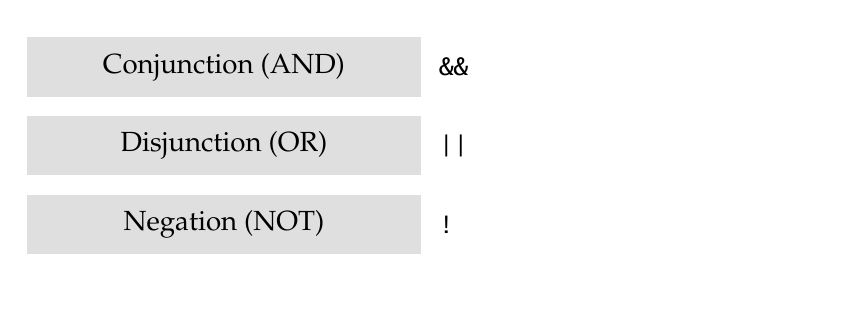
\begin{tikzpicture}
    \path[use as bounding box] (-5,.5) rectangle (5,-3);
    \node[anchor=east,item,minimum width=5cm] at (0,0) {Conjunction (AND)};
    \node[anchor=west] at (0.1,0) {\tt \&\&};
    \node[anchor=east,item,minimum width=5cm] at (0,-1) {Disjunction (OR)};
    \node[anchor=west] at (0.1,-1) {\tt ||};
    \node[anchor=east,item,minimum width=5cm] at (0,-2) {Negation (NOT)};
    \node[anchor=west] at (0.1,-2) {\tt !};
  \end{tikzpicture}
\end{center}



\end{document}